% !TeX spellcheck = da_DK
\section{Sensorer}
Følgende afsnit vil undersøge de sensorer der er interessante for dette projekt.
Da der er stor forskel på sensorerne der er tilrådighed er der foretaget forskellige forsøg, hvis formål er at klarlægge præcisionen af de forskellige sensorer.
Disse vil samtidig blive holdt op imod de forsøg der er blevet udført i \citet{tikNXT}, på de samme sensorer.

\subsection{Ultrasonic Sensor}
Ultrasonic sensoren (US), som kan ses på \cref{sensor:ultrasonic_sensor}, er en sensor der kan måle afstande til objekter.

\begin{figure}[h]
\centering
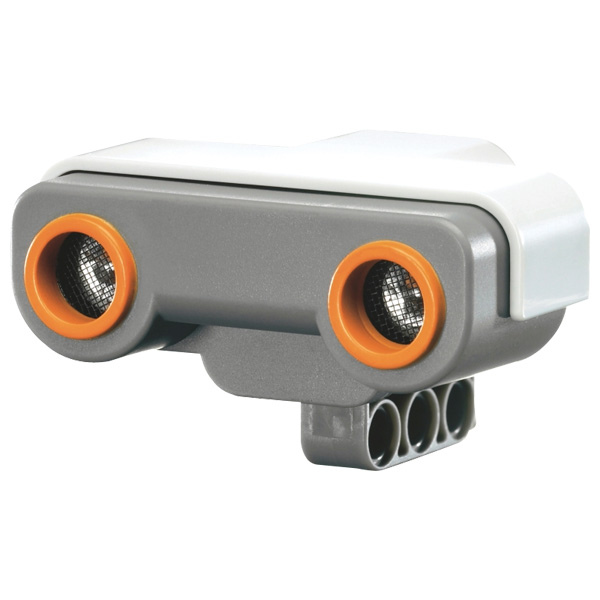
\includegraphics[width=.5\textwidth]{us}
\caption{\legoms Ultrasonic Sensor}
\label{sensor:ultrasonic_sensor}
\end{figure}

Det gøres ved at sende en lydbølge, hvorefter der beregnes hvor lang tid det tager for denne at ramme objektet, for derefter at blive reflekteret tilbage igen.
Sensoren måler afstanden i cm eller tommer.
Den maksimale afstand der kan måles er 255 cm, med en præcision på $\pm$3 centimeter.\cite{tikNXT}

\paragraph{Eksperimenterne i \citet{tikNXT}} har vist at \thilemann{En anden løsning på henvisninger til kilden?}
\begin{itemize}
\item den minimale aftsand der kan måles er 3 cm.
\item det bedst genkendelig objekt er firkantet med en glat og hård overflade.
\item desto mindre objektet er, desto sværere har sensoren ved at se det.
\item Sensorens højre 'øje' er det der sender lydbølgen, mens det venstre modtager.
Det betyder at sensoren 'ser' bedre i højre side når den befinder sig i horisontal position.
Dette ses tydeligt når afstand mellem sensor og objekt er under 20 cm, da den således ikke ligger indenfor sensorens synsfelt.
\item anvendes sensoren i vertikal position kan den blive distraheret af underlaget når bølgerne reflekteres tilbage til sensoren.
\end{itemize}

\paragraph{Den bedste opstilling} for sensoren er når den bruges i horisontal position
Det giver de bedste resultater, fordi den kritiske region ifht. den vertikale position er mindre.
En vinkel på mere end 15 grader fra lydbølgen giver hellere ikke klare resultater. \thilemann{Måske en illustration af hvad der menes?}
Desuden er runde genstande også svært genkendelige for sensorens synsfelt. \thilemann{Hvorfor?}

\subsubsection{Test}
Der er gennemført en mindre test af sensoren, for at svare på følgende spørgsmål:

\begin{itemize}
\item Hvor langt rækker sensoren i praksis?
\item Hvor stor nøjagtighed har den i praksis?
\item Ligner resultaterne dem fra eksperimenterne ovenfor?
\end{itemize}

\paragraph{Opstillingen} som blev brugt til at svare på disse spørgsmål kan ses i \cref{sensor:ultrasonic_opstilling}, bestående af: 

\begin{tabular}{|l|}
\hline
Tommestok\\
\hline
NXT 2.0\\
\hline
\legoms Ultrasonic Sensor\\
\hline
\legoms kabel.\\
\hline
\end{tabular}
\paragraph{}
Tommestokken blev brugt til at måle den nøjagtige afstand og derefter blev sensoren aflæst.
\mikael{Er det vigtigt med et billede af opstillingen? Er det ikke nok bare at beskrive den?}
\bruno{skal evt. i appendix}

\begin{figure}[h]
\centering
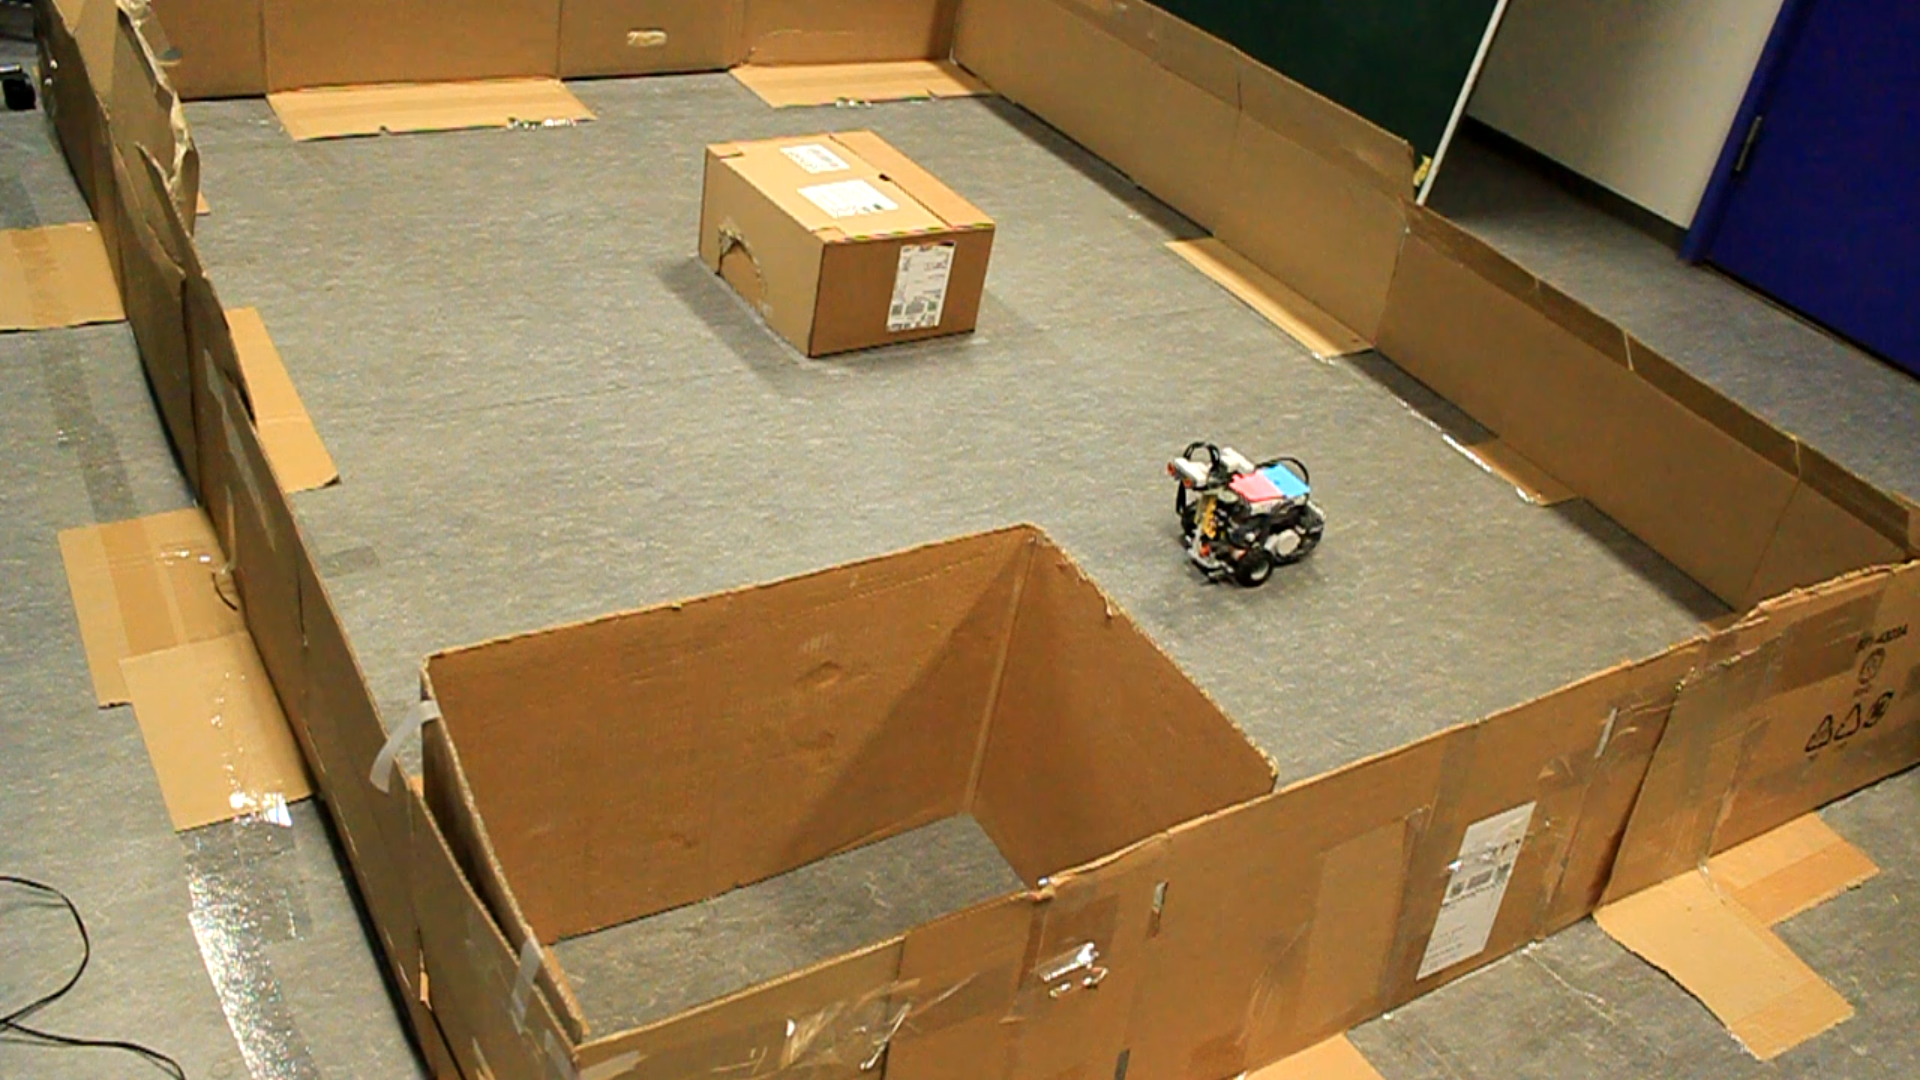
\includegraphics[width=.6\textwidth]{opstilling}
\caption{Forsøgsopstilling for test af US'ens afstands præcision}
\label{sensor:ultrasonic_opstilling}
\end{figure}

\begin{figure}[h]
\centering
\begin{tabular}{r | c | c | c |}
optimal & test1 & test2 & test3 \\
\hline
1 & 6 & 6 & 6 \\
10&	22&	23&	23\\
20&	22&	23&	23\\
30&	31&	31&	32\\
40&	40&	41&	40\\
50&	50&	50&	51\\
60&	60&	61&	61\\
70&	70&	71&	66\\
80&	80&	81&	81\\
90&	90&	91&	91\\
100&	100&	101&	102\\
110&	111&	112&	112\\
120&	120&	121&	121\\
130&	131&	131&	131\\
140&	141&	141&	141\\
150&	151&	151&	151\\
160&	161&	161&	163\\
170&	171&	171&	171\\
180&	255&	181&	181\\
190&	255&	190&	191\\
200&	202&	201&	202\\
210&	255&	255&	213\\
220&	255&	255&	222\\
230&	255&	255&	232\\
240&	255&	255&	255\\
250&	255&	255&	255\\
260&	255&	255&	255\\
\end{tabular}
\caption{Forsøgsresultater: afstande til objekt i cm.}
\label{sensor:ultrasonic_test_data}
\end{figure}

\paragraph{Resultaterne} fra forsøget kan ses i \cref{sensor:ultrasonic_test_data}.
I \cref{sensor:ultrasonic_resultat_diagram} ses hvordan at de tre tests alle giver forkerte resultater når sensoren er mindre en 20 cm fra objektet.
Desuden kan det ses på \cref{sensor:ultrasonic_resultat_diagram} at der i test1 kun kunne måles op til 170 cm før der opstod usikkerhed, hvor de andre tests nåede 200 (test2) og 230 (test3) cm før der opstod større usikkerhed.
Generelt holder det som der bliver lovet, nemlig at der er en afvigelse på 3 cm på målingerne, men forsøget viser at der kun med sikkerhed kan måles mellem 20 og 170 cm.

\begin{figure}[h]
\centering
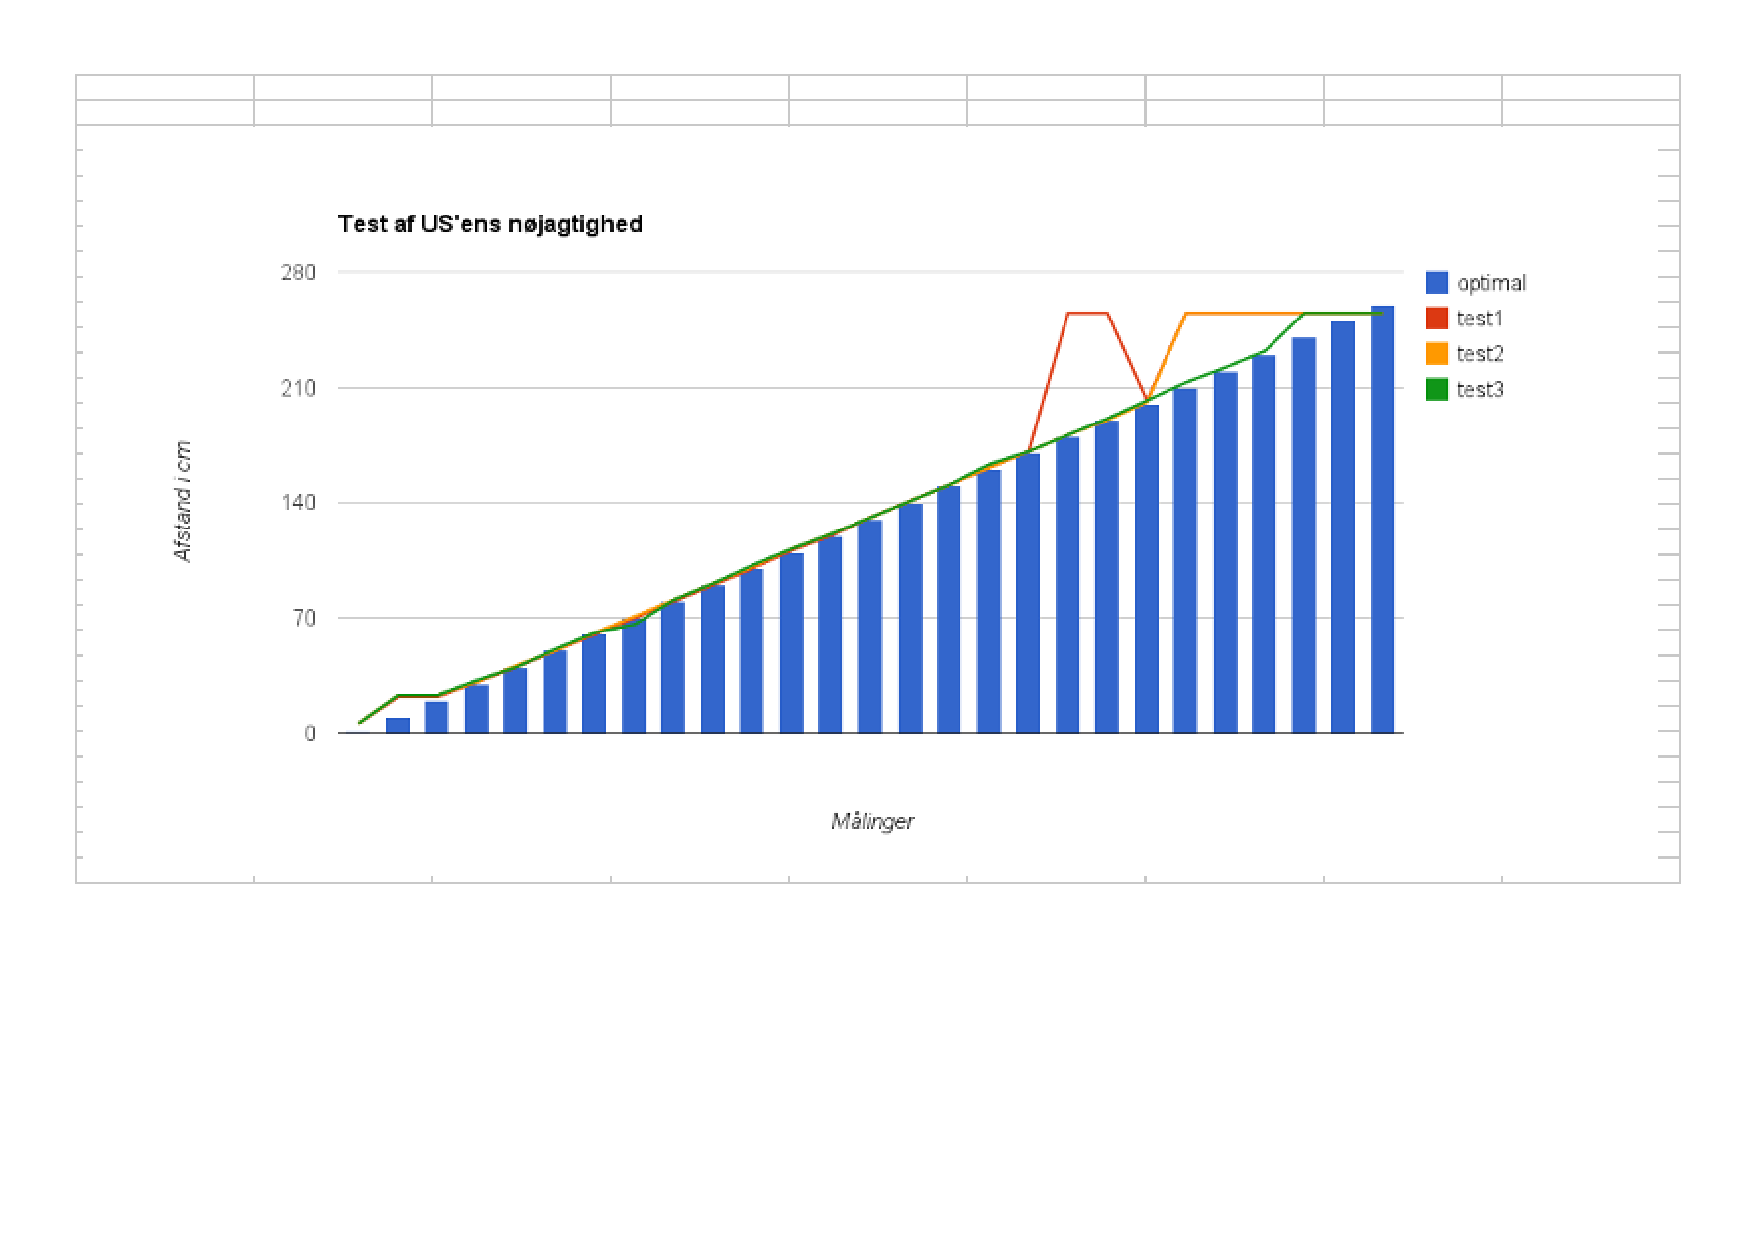
\includegraphics[width=\textwidth]{us_result_diagram}
\caption{Testresultater: De blå søjler repræsenterer den målte afstand med tommestok, de andre tre viser US'ens testresultater ifht. hianden.}
\label{sensor:ultrasonic_resultat_diagram}
\stefan{Ændr US'en til sensoren}
\end{figure}



\subsection{Infarød Sensor}
Den infarøde afstandssensor (IS) som kan ses på \cref{sensor:infraroed_sensor} er en afstandssensor med høj præcision og et interval på 10 til 80 cm.
\bruno{sensor not working at the moment :i}

\begin{figure}[h]
\centering
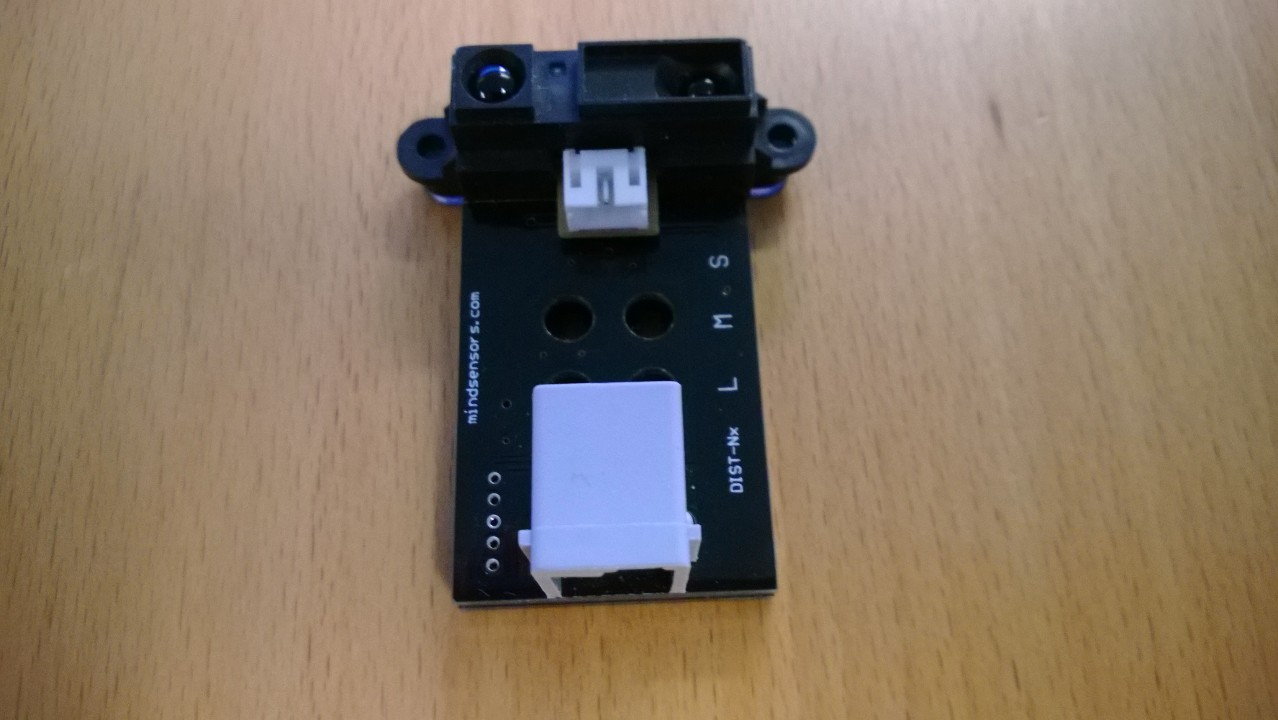
\includegraphics[width=.5\textwidth]{is} 	
\caption{High Precision Medium Range Infrared Distance Sensor for NXT (v2)}
\label{sensor:infraroed_sensor}
\end{figure}

\subsection{Motor}
Motoren beskrevet i dette afsnit er \lego's egen.
Den består af en rotationssensor som måler omdrejningerne ved grader med en nøjagtighed på 1 grad, hvilket er med til at gøre motoren ret præcis. 
Desuden gør denne sensor det også muligt at styre hvor meget kraft motoren skal køre med.
Kører med flere motorer har NXT'en indbygget software der gør det muligt at synkronisere disse, hvilket er smart hvis den ene motor skulle være stærkere eller svagere end den anden.\cite{tikNXT}
Motoren kan ses på \cref{sensor:motor_sensor}.
\\

\begin{figure}[h]
\centering
%http://www.philohome.com/nxtmotor/nxtmotor.htm
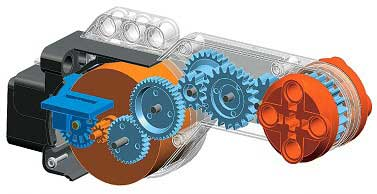
\includegraphics[width=.5\textwidth]{motor} 	
\caption{\legoms Servo Motor}
\label{sensor:motor_sensor}
\end{figure}

\paragraph{Eksperimenterne i \citet{tikNXT}} har vist at
\begin{itemize}
\item ved forsøg med en TriBot hvor den skal køre samme vej tilbage som den kom fra, rammer den flere centimeter ved siden af.
\item antallet af centimeter den afviger i førnævnte punkt stiger med afstanden og omvendt. \stefan{Hvad betyder ``og omvendt'' helt præcist?}
\item der er konstateret en afvigelse på $\pm$2 grader, som fortæller os hvorfor TriBot forsøget afviger med flere centimeter.
\item på trods af den indbyggede rotationssensor har motorerne ikke god præcision.
\end{itemize}

\subsubsection{Test}
Der er gennemført en test af motoren, for at svare på følgende spørgsmål:

\begin{itemize}
\item Kan det virkelig passe at den har 1 grads nøjagtighed?
\item Hvad er den praktiske nøjagtighed?
\item Giver motorerne det samme resultat når de er synkroniserede?
\end{itemize}

\paragraph{Opstillingen} brugt for at svare på disse spørgsmål kan ses på \cref{sensor:motor_sensor_opstilling}.
\mikael{Er det nødvendigt at vise opstillingen? Er det ikke nok bare at beskrive den?}

\begin{figure}[h]
\centering
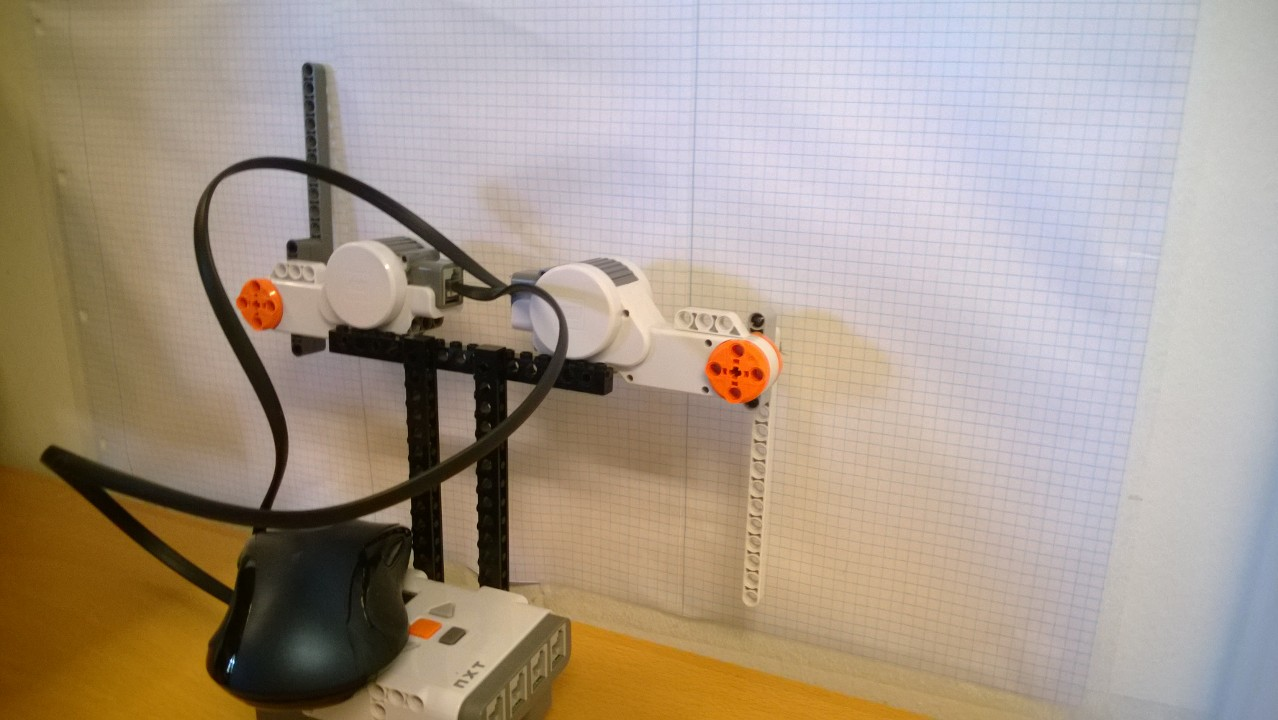
\includegraphics[width=.75\textwidth]{motor_opstilling} 	
\caption{Forsøgsopstillingen for nøjagtighedstesten af motoren.}
\label{sensor:motor_sensor_opstilling}
\end{figure}

Forsøgsopstillingen består af følgende dele:

\begin{tabularx}{\textwidth}{|X|X|}
\hline
NXT v2 & 3 A4 ark(ternet)\\
\hline
2x \legoms motor sensor & Tape\\
\hline
2x \legoms kabler & Vinkelmåler\\
\hline
LEGO & Stiftblyant\\
\hline
\end{tabularx}

\paragraph{}

Opstillingen blev bygget efter følgende fremgangsmåde:

\begin{enumerate}
\item Der startes med at bygge et stativ til de to motorer på NXT'en.
\item Derefter sættes de to motorer på stativet og forbindes vha. kablerne til NXT'en (Med en mus modvægt (\cref{sensor:motor_sensor_opstilling}), så NXT'en ikke vælter).
\item De tre A4 ark sættes op på en væg så motoren er centreret ud fra papirets højde.
\item En forlænger sættes på de to motorer, så den holder sig over papiret på en omdrejning.
\item Afmærk midten af motoren på papiret ved at sætte en stiftblyant igennem midten af motorens akse.
\end{enumerate}

\paragraph{}
Sådan blev forsøget gennemført:

\begin{enumerate}
\item Sæt motoren i gang og afmærk hvor forlængeren stopper.
\item Det afmærkede midterpunkt bliver brugt til at måle vinklen til det afmærkede punkt ud for forlængeren.
\item Tacho-værdien (antal grader drejet) noteres. 
Denne værdi kan læses ud af motorens rotationssensor vha. software.
\end{enumerate}

\begin{figure}[h]
\centering
\begin{tabular}{r | c | c | c | c | r |}
grader sat & \parbox{2.5cm}{motor b \\ grader målt*} & \parbox{2.cm}{motor b \\ tacho slut**} &  \parbox{2.5cm}{motor b \\ grader målt*} & \parbox{2.5cm}{motor b \\ tacho slut**} & optimal \\
\hline
1&	1&	0&	1&	0&	1\\
2&	2&	2&	2.5&	2&	2\\
3&	2&	3&	3&	3&	3\\
4&	5&	4&	4&	3&	4\\
5&	5&	6&	4&	4&	5\\
10&	10&	9&	9&	10&	10\\
15&	11&	16&	14&	15&	15\\
20&	20&	20&	18&	20&	20\\
25&	21&	25&	23&	25&	25\\
50&	57&	50&	56&	50&	50\\
75&	80&	77&	80&	79&	75\\
100&	100&	99&	95&	100&	100\\
150&	150&	149&	145&	150&	150\\
200&	204&	197&	200&	199&	200\\
400&	400&	401&	400&	398&	400\\
800&	799&	800&	800&	799&	800\\
1200&	1204&	1201&	1200&	1200&	1200\\
1800&	1796&	1796&	1799&	1800&	1800\\
3600&	3601&	3600&	3597&	3599&	3600\\

\end{tabular}
\caption{Forsøgsresultater for motor nøjagtighedstesten.}
\label{sensor:motor_test_data}
\end{figure}

\paragraph{Resultaterne} fra forsøget kan ses på \cref{sensor:motor_test_data}.
Hvis vi kigger på \cref{sensor:motor_test_data} kan vi bestemme den største afvigelse til +7 og -4 grader målt.
Tacho-værdien har en afvigelse på maksimalt +1 og -4 grader.
Dette stemmer ikke overens med de antagede $\pm$1 grad afvigelse.

+7 og +6 grader målt optræder kun en gang.
Ellers er den maksimale målte afvigelse $\pm$4 grader, men selvom vi antager at det er pga. unøjagtige målinger ved forsøgsudførelsen, er det stadig ikke $\pm$1 grad.
\stefan{Man kan ikke direkte aflæse afvigelserne fra tabellen}
\thilemann{Synes heller ikke meningen står helt klar}
Kigger vi på \cref{sensor:motor_sensor_diagram1} kan vi se at målingerne ligger længst udenfor det optimale (sorte stiplede linje), hvilket er en god indikator på at det er bedre at benytte tacho-værdien.

Desuden kan vi se på samme figur at motor b er meget mere unøjagtig end motor c.
Ideelt ville de to motorer give det samme resultat.

Dvs. den målte værdi har en afvigelse på $\pm$4 grader, mens tacho-værdien har en afvigelse på +1 og -4 grader, og at synkronisering af de to motrer ikke giver den ønskede effekt.

\begin{figure}[h]
\centering
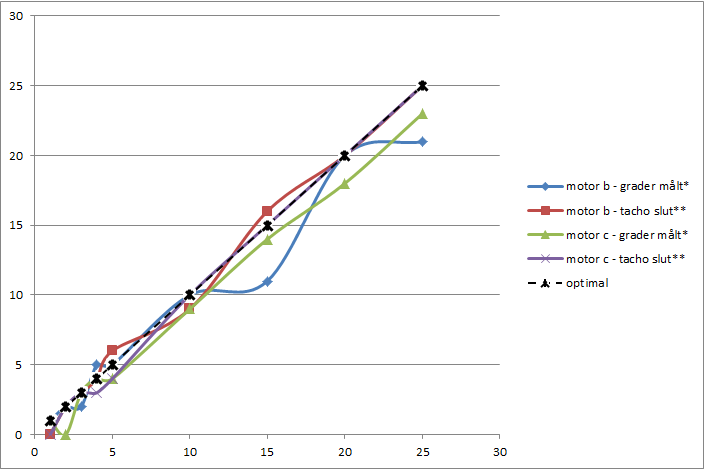
\includegraphics[width=.75\textwidth]{motor_diagram1} 	
\caption{Forsøgsdiagram for forsøget omkring motorens nøjagtighed, grader 0 til 50.}
\label{sensor:motor_sensor_diagram1}
\end{figure}

\begin{figure}[h]
\centering
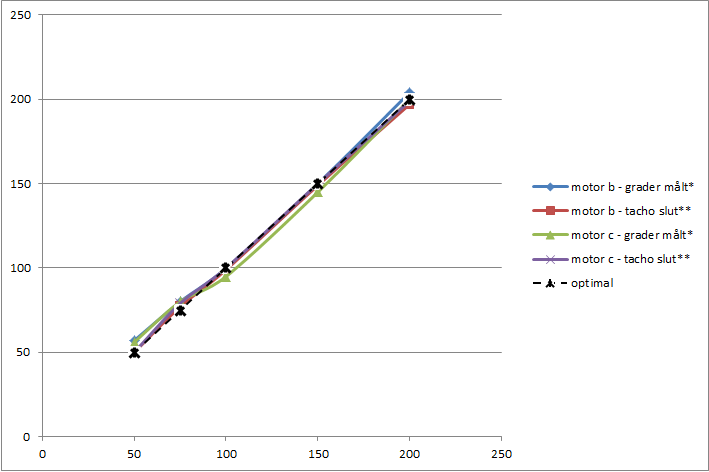
\includegraphics[width=.75\textwidth]{motor_diagram2} 	
\caption{Forsøgsdiagram for forsøget omkring motorens nøjagtighed, grader 50 til 200.}
\label{sensor:motor_sensor_diagram2}
\bruno{Ikke brugt i teksten, kan være den bare skal smides ud}
\stefan{grafen er meget upræcis at aflæse}
\end{figure}

\begin{figure}[h]
\centering
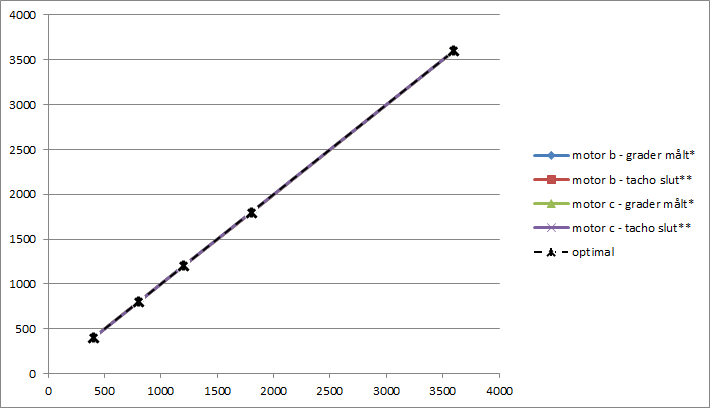
\includegraphics[width=.75\textwidth]{motor_diagram3} 	
\caption{Forsøgsdiagram for forsøget omkring motorens nøjagtighed, grader 200 til 3600.}
\label{sensor:motor_sensor_diagram3}
\bruno{Ikke brugt i teksten, kan være den bare skal smides ud}

\end{figure}